%-----------------------------------------------
% Template para criação de resumos de projectos/dissertação
% jlopes AT fe.up.pt,   Fri Jul  3 11:08:59 2009
%-----------------------------------------------

\documentclass[9pt,a4paper]{extarticle}

%% English version: comment first, uncomment second
%\usepackage[portuguese]{babel}  % Portuguese
\usepackage[english]{babel}     % English
\usepackage{graphicx}           % images .png or .pdf w/ pdflatex OR .eps w/ latex
\usepackage{times}              % use Times type-1 fonts
\usepackage[utf8]{inputenc}     % 8 bits using UTF-8
\usepackage{url}                % URLs
\usepackage{multicol}           % twocolumn, etc
\usepackage{float}              % improve figures & tables floating
\usepackage[tableposition=top]{caption} % captions
%% English version: comment first (maybe)
%\usepackage{indentfirst}        % portuguese standard for paragraphs
%\usepackage{parskip}

%% page layout
\usepackage[a4paper,margin=30mm,noheadfoot]{geometry}

%% space between columns
\columnsep 12mm

%% headers & footers
\pagestyle{empty}

%% figure & table caption
\captionsetup{figurename=Fig.,tablename=Tab.,labelsep=endash,font=bf,skip=.5\baselineskip}

%% heading
\makeatletter
\renewcommand*{\@seccntformat}[1]{%
  \csname the#1\endcsname.\quad
}
\makeatother

%% avoid widows and orphans
\clubpenalty=300
\widowpenalty=300

\begin{document}

\title{\vspace*{-8mm}\textbf{\textsc{Explorando Conceitos de Programação Visual\\para Programação Probabilística}}}
\author{\emph{Gabriel Cardoso Candal}\\[2mm]
\small{Dissertação realizada sob a orientação de \emph{Prof.\ Hugo Sereno Ferreira}}}
\date{}
\maketitle
%no page number
\thispagestyle{empty}

\vspace*{-4mm}\noindent\rule{\textwidth}{0.4pt}\vspace*{4mm}

\begin{multicols}{2}

\section{Motivação}

Existe, entre vários domínios com problemas relevantes e interessantes para resolver
(visão por computador, criptografia, biologia, deteção de fraude, sistemas de recomendação,
...) \cite{intml}, a necessidade recorrente de tomar decisões em ambientes de incerteza
usando métodos de \textit{machine learning}.

Um dos métodos de ML que pode ser usado para abordar este problema é construir um
modelo probabilístico através uso de uma linguage de programação probabilística,
que permite definir um modelo como um programa e oferece inferência pronta a usar \cite{Prekopa2003}.
Apesar do poder e flexibilidade destas linguagens, é difícil para a sua audiência
(\textit{data scientists}, estátisticos, matemáticos, ...) adaptarem-se à representação
textual que estas linguagens oferecem, já que carecem da intuição gráfica dada
por outras ferramentas às quais estão habituados. Acreditamos que isto afeta
negativamente a produtividade e desacelera a adopção das linguagens de programação
probabilística \cite{darpa}.

\section{Objetivos}

Quisemos ultrapassar as dificuldades de aprender uma nova linguagem, tanto para
progrmaadores inexperientes como para os mais experientes, como aprender
uma nova sintaxe ou adapter aos idiomas de uma linguagem. É sabido que linguagens
típicas são difíceis de aprender e usar \cite{Lewis1987} e que existem vantagens em providenciar
uma linguagem com uma interface gráfica \cite{dfbeg}.

O objetivo desta dissertação foi desenvolver uma linguagem de Programação Visual (PV)
com capacidades de programação probabilística. A audiência são programadores e
\textit{data scientists} com conhecimentos em estatística que não estejam ainda
confortáveis com linguagens de programação probablística, mas desejam educar-se
neste tópico para que eventualmente possam tirar partido do poder desta nova abordagem
de \textit{machine learning}.

\section{Descrição do trabalho}

Durante esta dissertação desenvolvemos um Ambiente de Programação Visual (APV),
uma ferramente que permite ao utilizador desenhar o seu modelo graficamente e
depois ou executá-lo ou transoformá-lo em código.

Ao fazê-lo providenciamos uma ferramente que pode ser usada para fazer investigação
de usabilidade. Por exemplo, permite estudos futuros em que seja avaliado empiricamente
se realmente pessoas com conhecimento de estatística aprendem mais rápido a usar
uma linguagme de programação probabilística usando o APV em vez da forma textual.
Também mostramos ser possível representação um programa probabilístico de forma gráfica
representando na nossa ferramenta alguns exemplos existentes em Infer.NET,
estando um deles representado na Fig. \ref{fig:first}.

\begin{figure}[H]
\centerline{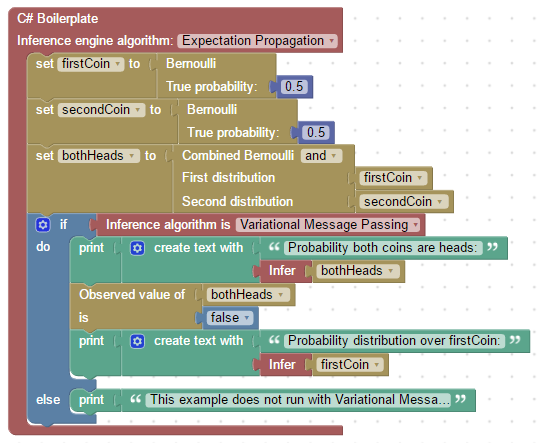
\includegraphics[scale=.6]{firstExample.png}}
\caption{Exemplo de um modelo probabilístico no nosso ambinete.}
\label{fig:first}
\end{figure}

During this process, we had to make choices regarding both the paradigms and the
technologies in which we would base our VPE on, and we
describe some of them below. In addition to detailing those choices, we are
using the remainder of this section to elicit some VP concepts
we find useful to have in a VP language for probabilistic programming.

\subsection{Puramente Visual \textit{vs} Ambiente}

A diferença entre um APV e uma linguagem puramente visual é que, enquanto a segunda
é uma linguagem \textit{per se} (ou seja, há uma mapeamento direto entre os
gráficos e a execução), os APV oferecem um meio termo entre linguagens textuais
e puramente visuais: providenciam uma interface gráfica que pode ser usada para
gerar código na linguagem alvo \cite{Burnett1999}. Estes dois conceitos são
normalmente referidos na literatura como se fossem mutualmente exclusivos,
mas incluímos ambos: temos um APV que pode executar código, para que o utilizador
possa ter \textit{feedback} visual o mais cedo possível (não é necessário copiar
o código para um ambiente diferente), o que é algo essencial em PV \cite{Shu1988}.

\subsection{\textit{Dataflow vs Blockly}}

Ao ter que escolher como representar visual a linguagem, tivemos que optar entre
duas alternativas. Enquanto programação \textit{dataflow} é usada em aplicações
comerciais bem sucessidades como \textit{RapidMiner} ou \textit{Blender}, representações \textit{à Blockly}
são mais vistas em ferramentas educacionais como o \textit{Scratchy} do MIT.

Por causa da natureza da nossa audiência, pensamos que seria adequado para a nossa
ferramente oferecer uma representação que pudesse gerar código mais semelhante
ao escrito por pessoas, para que os utilizadores pudessem olhar para a nossa ferramente
como uma rede de segurança para gerar código como se fossem eles a tê-lo escrito,
até que fossem proficientes o suficiente para que não precisassem do APV. Devido
a isto, decidimos usar uma representação \textit{à Blockly}.

\subsection{Conceitos de Programação Visual}

Há um conjunto de conceitos de programação visual que parece ser essencial
incluir para que os utilizadores possam ser mais rápidos e cometer menos
erros aquando do desenvolvimento recorrendo a uma ferramente de PV, tais como:

\begin{itemize}
  \item Comentários
  \item Duplicação de blocos
  \item Procurar blocos por nome
  \item Usar cores e ícones para transmitir significados
  \item Obter ajuda (ver detalhes da funcionalidade de um bloco)
  \item Serialização (gravar e carregar programas e também pode partilhá-los)
  \item Zoom, minimização e compressão de blocos (minimizar espaço utilizado quando os detalhes não importam)
\end{itemize}

\subsection{Segurança de tipos}

Devido a estarmos a usar um APV baseado em representações \textit{à Blockly},
que é mais adequado para propósitos educacionais, é da maior importância ter
segurança de tipos. Isto quer dizer que, além de não ser possível representar
um programa com erros de sintaxe, também não é possível cometer erros de tipos
(tais como usar um valor booleano para especificar a média de uma distribuição
gaussiana).
Isto é feito de forma natural: tal como num puzzle, blocos que violem as regras
de tipos não encaixam. Esta abordagem é melhor do que esperar para ver erros
de compilação ou de tempo de execução, já que o erro é apanhado mais cedo e o
\textit{feedback} visual é mais imediato.

\section{Conclusões}\label{sec:conclui}

É nossa crença que a representação gráfica é mais clara do que o seu dual textual,
principalmente porque os parâmetros têm nomes e existem cores.

A maior razão para usar um APV ao invés da representação textual original é devido
à rede de segurança que providencia e impede o utilizador de cometer certos erros.
Por causa disto, acreditamos que este tipo de APV pode ser útil para ajudar
\textit{data scientists} que são inexperientes a programar a dar os primeiros passos
no uso de uma linguagem de programação probabilística.

Contudo, se não olharmos para o APV como uma ferramente educacional mas sim como
algo que não é transacional, pensamos que não é tão produtivo quando comparado com
ferramentas como \textit{RapidMiner}, \textit{Excel} ou mesmo representações textuais.
O maior motivo por trás disto tem a ver com o uso de uma representação \textit{à Blockly}
que faz com que não tenhamos uma linguagem puramente visual que não encapsula
totalmente os conceitos de programação textual (como a declaração de variáveis).
No caso de existir alguém a considerar desenvolver uma linguagem de PV para ser usada
como substituto da forma textual de linguagens de programação probabilística,
aconselhamos a explorar uma representação \textit{dataflow}, já que funciona a um
nível de abstração mais alto e tem sido usado com mais sucesso em aplicação usadas
na indústria e na academia.

%%English version: comment first, uncomment second
\bibliographystyle{unsrt-pt}  % numeric, unsorted refs
%\bibliographystyle{unsrt}  % numeric, unsorted refs
\bibliography{refs}

\end{multicols}

\end{document}
